\documentclass[12pt]{article}
\usepackage[utf8]{inputenc}
\usepackage[T1]{fontenc}
\usepackage[french]{babel}
\usepackage{geometry}
\usepackage{listings}
\usepackage{xcolor}
\usepackage{graphicx}
\usepackage{hyperref}
\usepackage{enumitem}
\usepackage{titlesec}

\geometry{a4paper, margin=2.5cm}
\geometry{a4paper, padding=2.5cm}

\lstset{
    basicstyle=\ttfamily, backgroundcolor=\color{gray!10}, frame=single, breaklines=true
}

\title{Guide complet de la manipulation de notre application}
\author{ANGE FOKAM}
\date{30/06/2025}
\begin{document}
    \maketitle
    % Plan de travail
    \newpage
    \section*{Inroduction générale}
    \addcontentsline{toc}{section}{Introduction générale}
        \begin{itemize}[label=--]
            \item \textbf{Objectif du guide} : Explique comment déployer, manipuler et utiliser l'application.
            \item \textbf{Public cible} : Administrateur système future, développeurs futures, utilisateurs finaux.
            \item \textbf{Structure du document} : Deux sections principales : déploiement technique, puis utilisation par le tierce.
            \item \textbf{Prérequis généraux} : Accès réseau, identifiants, connaissances de base en informatique, connaissances de base en programmation.
        \end{itemize}
    % Pour les developpeurs
    \section{Guide de deploiement de l'application}
        \subsection{Matériel à disposer}
            \begin{itemize}[label=--]
                \item Configuration minimale recommandée
                \item Outils nécessaires (logiciels, bibliothèques, accès réseau, etc.)
            \end{itemize}
        \subsection{Installation des environnements}
            \begin{itemize}[label=--]
                \item Environnement de développement
                \item Environnement de test
                \item Étapes d’installation détaillées (avec commandes si besoin)
            \end{itemize}
        \subsection{Modification des variables d’environnement}
            \begin{itemize}[label=--]
                \item Variables nécessaires à définir
                \item Emplacement des fichiers de configuration
                \item Exemples de fichiers \texttt{.env} ou équivalents
            \end{itemize}
        \subsection{Déploiement des serveurs}
            \begin{itemize}[label=--]
                \item Lancement des services backend de l'application
                \item Lancement du frontend de l'application
                \item Vérification du bon fonctionnement des serveurs
            \end{itemize}
        \subsection{Ouverture de l’application}
            \begin{itemize}[label=--]
                \item URL d’accès
                \item Port(s) utilisé(s)
                \item Premier test de connexion à l’application
            \end{itemize}

    % Pour les utilisateurs
    \section{Guide d’utilisation de l’application}
        \subsection{Présentation de la page de connexion}
            \begin{itemize}[label=--]
                \item Capture d’écran (facultatif)
                \item Description des champs requis (nom d’utilisateur, mot de passe, etc.)
            \end{itemize}
        \subsection{Procédure de connexion}
            \begin{itemize}[label=--]
                \item Étapes de connexion pour un utilisateur
                \item Gestion des erreurs de connexion
                \item Réinitialisation de mot de passe (si applicable)
            \end{itemize}
        \subsection{Soumission d’un projet}
            \begin{itemize}[label=--]
                \item Accès à la fonctionnalité
                \item Champs à remplir
                \item Boutons/actions à déclencher
                \item Confirmation et suivi du projet
            \end{itemize}
        \subsection{Effectuer une requête}
            \begin{itemize}[label=--]
                \item Accéder à la fonctionnalité
                \item Paramétrer la requête
                \item Valider et visualiser les résultats
                \item Sauvegarder ou exporter une requête (si disponible)
            \end{itemize}

    \section*{Annexes}
        \addcontentsline{toc}{section}{Annexes}
            \begin{itemize}[label=--]
            \item Glossaire des termes techniques
            \item Contacts techniques pour assistance
            \item Liens utiles (dépôts Git, documentation externe, etc.)
        \end{itemize}

    \section*{Conclusion}
        \addcontentsline{toc}{section}{Conclusion}
            \begin{itemize}[label=--]
            \item Résumé des étapes importantes
            \item Conseils pour une bonne utilisation
            \item Mise à jour du guide (comment le maintenir à jour)
        \end{itemize}
        \newpage
        % Introduction
        \section*{Introduction générale}
        \addcontentsline{toc}{section}{Introduction générale}
            \noindent
            Dans le monde du développement, les applications doivent être entretenues au quotidien. 
            À cet effet, elles doivent être conçues de manière à ce que les générations futures puissent 
            facilement les maintenir en activité. De plus le developpement des aplications doivent palier
            aux besoins de ses utilisateurs. Demble, nous avons donc mis en place une série d'étapes pour 
            le lancement de notre application à partir d’un poste personnel, aussi bien pour les developpeurs 
            et administrateurs que pour les utilisateurs de l'aplications afin de pouvoir mieux l'utiliser
            au quotidien. Bien que ce processus puisse sembler complexe, il vise à faciliter la prise en
            main et la maintenance à long terme de l’application par les futurs intervenants, ainsi que la 
            gestion des projets de fin de cycle des etudiants. Pour une utilisation complete de l'application, 
            nous avons reparti la presentation en deux section, la premiere section qui expliquera comment
            les developpeurs et les Administrateurs systeme ferons leur part, et la deuxieme, qui presentera
            tous ce que les utilisateurs (etudiants, professeurs, visiteurs) doivent savoir et savoir faire 
            dans l'application.
            \vspace{0.5cm}
        % Section une
        \section{Guide de déploiement de l’application}
            \subsection{Matériel à disposer et prerequis}
            Avant de commencer l'installation, assurez-vous d'avoir les éléments suivants installés sur votre
            poste de travail : 
                \begin{itemize}[label=--]
                    \item PHP (Version 8.0 ou la plus récente)
                    \item Composer
                    \item Angular
                    \item Laravel 10+
                    \item VS code (De preference comme editeur de texte)
                    \item MySQL (Vous pouvez l'utiliser depuis l'application xampp)
                    \item Elasticsearch (Version compatible avec votre projet)
                    \item Git (Vous devez disposer d'un compte git pour effecteur votre travail d'equipe et d'autre taches...)
                \end{itemize}
            Pour ce qui est du matériel et les ressources nécessaires, vous devez procéder au déploiement :
            \begin{itemize}[label=--]
                \item \textbf{1. Configuration minimale recommandée} : 
                    \begin{itemize}
                        \item Processeur : 2 GHz double cœur ou plus
                        \item Mémoire RAM : 8 Go minimum
                        \item Stockage : 30 Go d’espace libre
                    \end{itemize}
                \item \textbf{2. Outils nécessaires} : 
                    \begin{itemize}
                        \item \texttt{Git}
                        \item Accès à Internet (Fia un fournisseur d'acces a internet ou un vpn)
                        \item Navigateur web à jour (Celui de votre choix telle que : microsoft edge, chrome, firefox, opera, avast ...)
                    \end{itemize}
            \end{itemize}
            \rule{linewidth}{0.3pt}
            Voici les étapes à suivre pour l’ouverture de notre projet (for windows and linux) :
            \begin{enumerate}
                \item \textbf{1. Cloner le dépôt GitHub}
                    \begin{itemize}
                        \item Cloner le dépôt Git :\\
                        \texttt{git clone https://github.com/Noobs440/UV_PROJET_AIGLE.git}
                    \end{itemize}
                \item \textbf{2. Configurer l’environnement}
                    \item Créez un fichier .env à partir du fichier exemple .env.example :
                        \begin{lstlisting}
                            Un exemple -> cp .env.example .env
                        \end{lstlisting}
                    \item Ouvrez le fichier .env dans un éditeur de texte et configurez les variables d'environnement suivantes :
                        \begin{lstlisting}
                            Base de Données :
                            DB_CONNECTION=mysql
                            DB_HOST=127.0.0.1
                            DB_PORT=3306
                            DB_DATABASE=nom_de_votre_base_de_donnees
                            DB_USERNAME=nom_utilisateur
                            DB_PASSWORD=mot_de_passe
                        \end{lstlisting}
                        \begin{figure}[h] 
                            \centering 
                            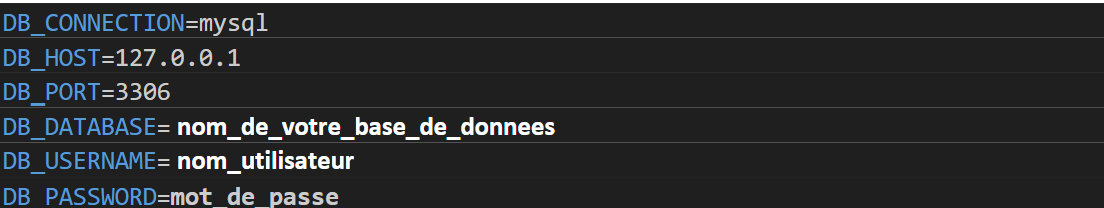
\includegraphics[width=0.6\textwidth]{./img/bd.png} 
                        \end{figure}
                    \item Elasticsearch :
                        \begin{figure}[h]
                            \centering
                            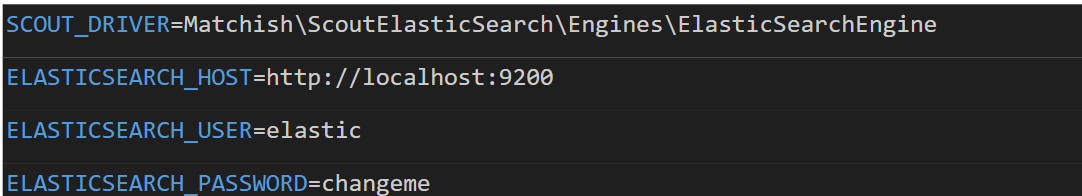
\includegraphics[width=0.6\textwidth]{./img/elas.png}
                        \end{figure}
                \item \textbf{3. Générer la Clé de l'Application}
                    \item Générez une nouvelle clé d'application en exécutant la commande suivante :
                    \begin{lstlisting}    
                        php artisan key:generate
                    \end{lstlisting}
                \item \textbf{4. Modification des variables d’environnement} 
                    \begin{figure}[h] 
                        \centering 
                        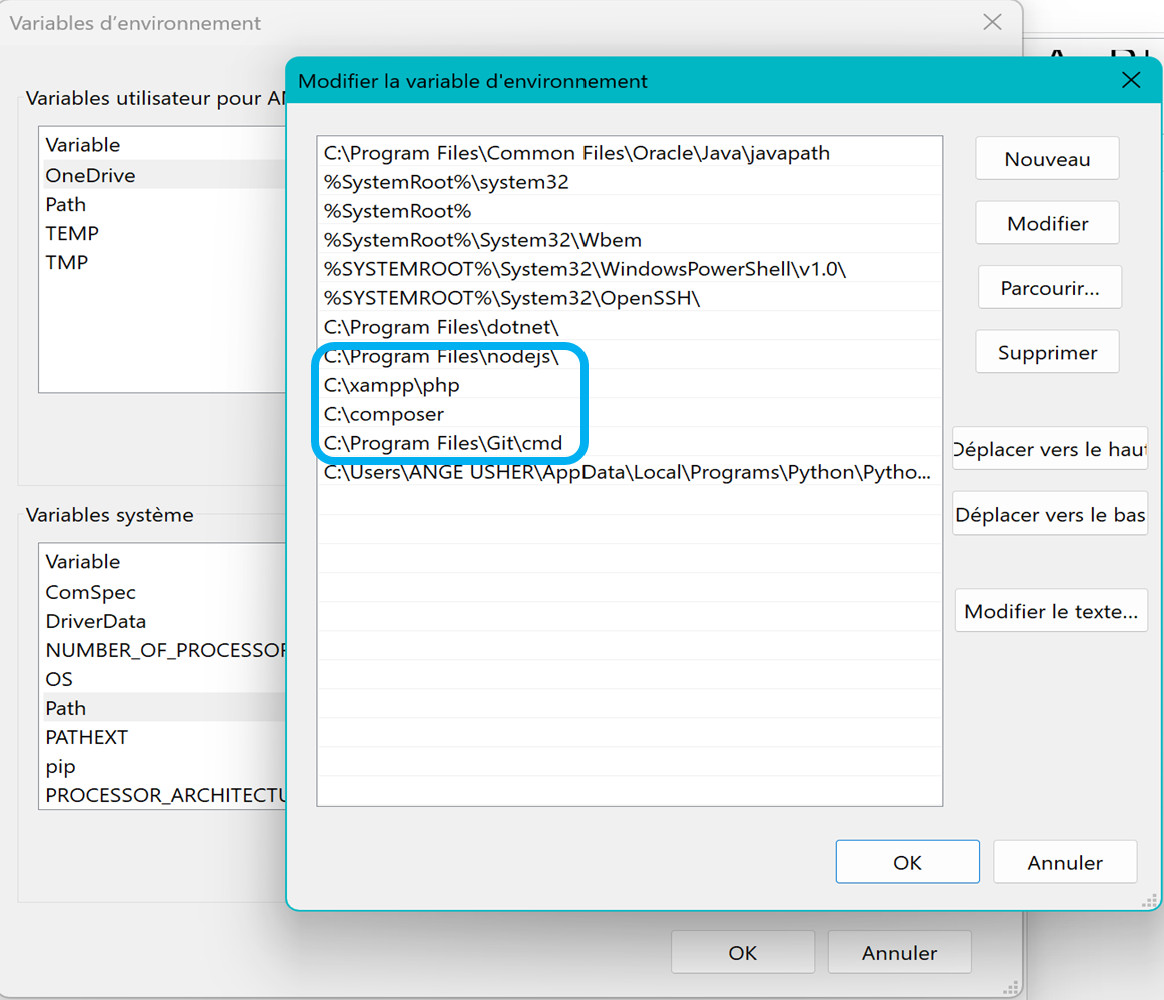
\includegraphics[width=0.6\textwidth]{./img/path.png} 
                    \end{figure}
                \item \textbf{{5. Installation et ouverture de XAMPP}, puis lancement des serveurs \textbf{Apache} et \textbf{MySQL}}
                    \begin{figure}[h] 
                        \centering 
                        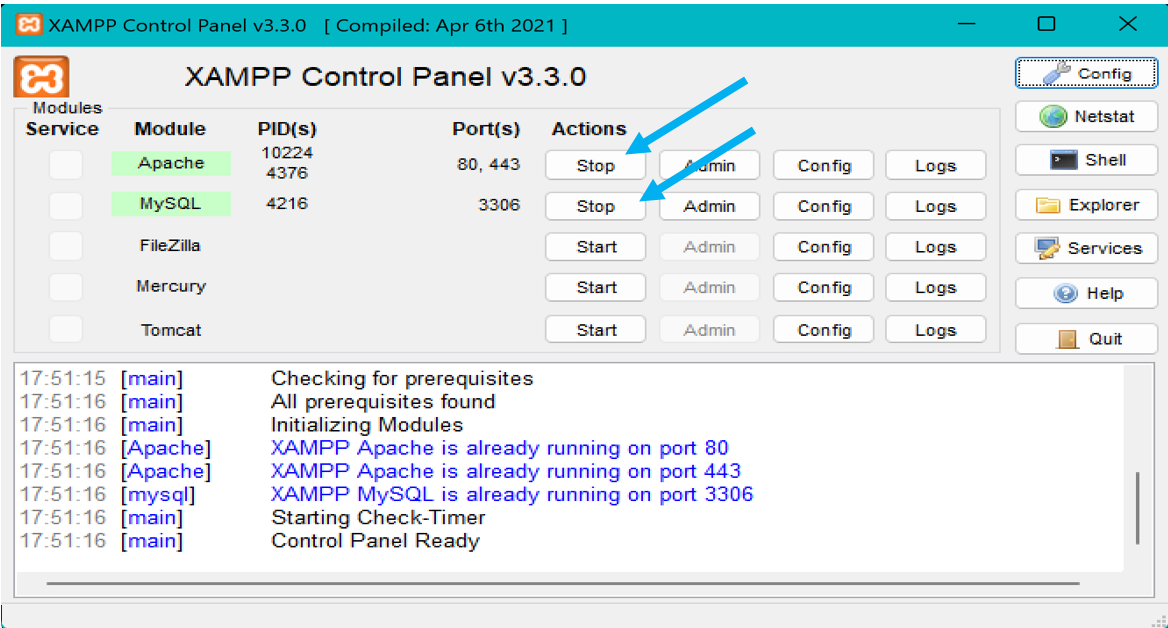
\includegraphics[width=0.6\textwidth]{./img/xampp.png} 
                    \end{figure}
                \item \textbf{6. Configurer la Base de données}
                    \item Créez la base de données dans MySQL que vous pouver nommer uv_projet_db, dans laquelle vous allez stoker toutes les informations relatives a l'application.
                \item \textbf{7. Installer et Configurer Elasticsearch}
                    \item 1. Téléchargez Elasticsearch depuis le site officiel.
                    \item 2. Extraire l'archive téléchargée dans un répertoire de votre choix.
                        \item nb: Remplacer le Fichier elasticsearch.yml
                    \item 3. Copiez le fichier elasticsearch.yml fourni dans le dépôt à l'emplacement de configuration d'Elasticsearch : 
                        Sur Windows
                            copy config\elasticsearch\elasticsearch.yml C:\chemin\vers\elasticsearch\config\
                          Assurez-vous de remplacer C:\chemin\vers\elasticsearch\ par le chemin réel où Elasticsearch est installé sur votre machine.
                        Sur Linux
                            cp config/elasticsearch/elasticsearch.yml /chemin/vers/elasticsearch/config/
                        Assurez-vous de remplacer /chemin/vers/elasticsearch/ par le chemin réel où Elasticsearch est installé sur votre machine
                \item \textbf{8. Ouvrez l'invite de commande (Cmd) en tant qu’administrateur ou pas, pour démarrer Elasticsearch}
                    \item Accédez au répertoire d'installation d'Elasticsearch et exécuter la commande qui suit :
                    \begin{lstlisting}
                        cd chemin\vers\elasticsearch-8.14.1
                        ./bin/elasticsearch.bat sur windows
                        ./bin/elasticsearch sur linux
                    \end{lstlisting}
                    \begin{figure}[h] 
                        \centering 
                        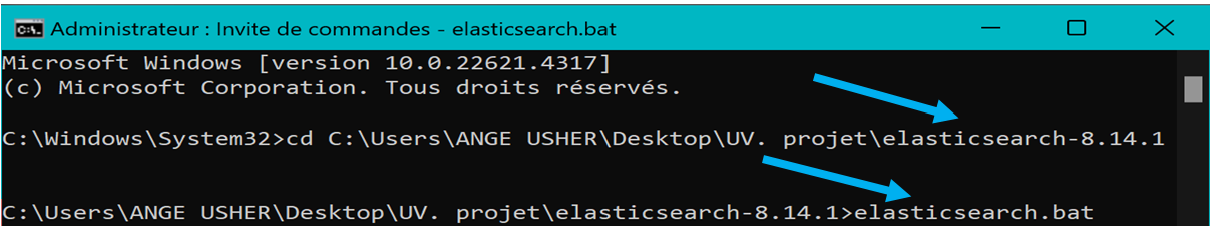
\includegraphics[width=0.6\textwidth]{./img/elastix.png} 
                    \end{figure}
                \item \textbf{9. Deploiyer le serveur de développement Laravel sur un second cmd (Celui de vs code de preference)}
                    \begin{itemize}
                        \item Entrer le chemin d’accès au dossier backend dans votre terminal :
                            \begin{lstlisting}
                                cd C:\chemin\vers\backend\laravel
                            \end{lstlisting}
                        \item Faire la migration des tables de l'applications dans la base de données que vous avez créer a l'etape précédentes :
                            \begin{lstlisting}
                                php artisan migrate:refresh --seed
                            \end{lstlisting}
                        \item Lancer le serveur Laravel :
                            \begin{lstlisting}
                                php artisan serve
                            \end{lstlisting}
                    \end{itemize}
                \item \textbf{10. Lancer le frontend Angular sur un troisieme cmd}
                    \item Entrer le chemin d’accès au dossier frontend dans votre terminal :
                    \begin{lstlisting}
                        cd chemin\vers\le\frontend
                    \end{lstlisting}
                    \item Entrer la commande :
                    \begin{lstlisting}
                        ng serve
                    \end{lstlisting}
                    L'applcication va commencer a builder et puis vous verez a la fin de l'operation :
                    \begin{figure}[h] 
                        \centering 
                        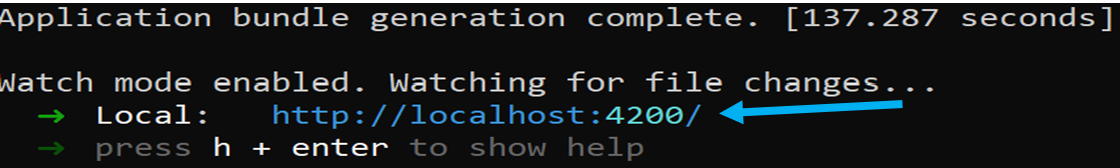
\includegraphics[width=0.6\textwidth]{./img/angular.png} 
                    \end{figure}
                    \item Enfin, copiez le lien d'accès local suivant dans votre navigateur :
                        \begin{lstlisting}
                            Local : http://localhost:4200/
                        \end{lstlisting}
            \end{enumerate}
            \begin{itemize}
                \item Problèmes Courants
                \begin{enumerate}
                    \item \textbf{Erreurs de Connexion à la Base de Données :}Vérifiez les paramètres de votre base de données dans le fichier .env.
                    \item \textbf{Problèmes avec Elasticsearch :}Assurez-vous qu'Elasticsearch est bien démarré et que le port est correctement configuré.
                \end{enumerate}
            \end{itemize}
        \rule{linewidth}{0.3pt}
        
        
        % Section deux



\end{document}